% =====================================================================
%  Prabhavit Gupta - Tailored CV for DevOps & Automation Engineer at Cognizant
%  Target: Cognizant Sweden (Energy & Utilities / GE ADMS Series 6)
%  Compile: tectonic cv/main_Cognizant_DevOps.tex
%  Rules: ONE PAGE. 0 em-dashes. Verified facts. ATS-optimized.
% =====================================================================
\documentclass[a4paper,10pt]{article}

\usepackage[T1]{fontenc}
\usepackage[utf8]{inputenc}
\usepackage[top=0.72cm,bottom=0.72cm,left=1.0cm,right=1.0cm]{geometry}
\usepackage{titlesec}
\usepackage{enumitem}
\usepackage{hyperref}
\usepackage{xcolor}
\usepackage{graphicx}

\definecolor{accent}{HTML}{1F4E78}
\hypersetup{colorlinks=true, urlcolor=accent, linkcolor=accent}
\pagestyle{empty}
\setlength{\parindent}{0pt}

\titleformat{\section}{\large\bfseries\color{accent}}{}{0em}{}[\vspace{-0.6em}\rule{\textwidth}{0.8pt}]
\titlespacing{\section}{0pt}{2pt}{1pt}

\newcommand{\role}[4]{%
 \textbf{#1} \hfill \textbf{#2}\\[1pt]%
 \textit{#3} \hfill \textit{#4}\\[2pt]%
}
\setlist[itemize]{leftmargin=1.2em, itemsep=0pt, topsep=1pt, parsep=0pt}

\begin{document}

% ================= HEADER =================
\begin{minipage}[c]{0.80\textwidth}
 {\Huge\bfseries Prabhavit Gupta}\\[3pt]
 {\color{accent}\large DevOps \& Automation Engineer: CI/CD, IaC \& Platform Reliability}\\[6pt]
 {\footnotesize +39 351 610 7807 ~$\vert$~
 \href{mailto:prabhavitg@gmail.com}{prabhavitg@gmail.com} ~$\vert$~
 \href{https://www.linkedin.com/in/prabhavit/}{linkedin.com/in/prabhavit} ~$\vert$~
 \href{https://github.com/prab-gupta}{github.com/prab-gupta} ~$\vert$~
 Venice, Italy}
\end{minipage}\hfill
\begin{minipage}[c]{0.18\textwidth}
 \raggedleft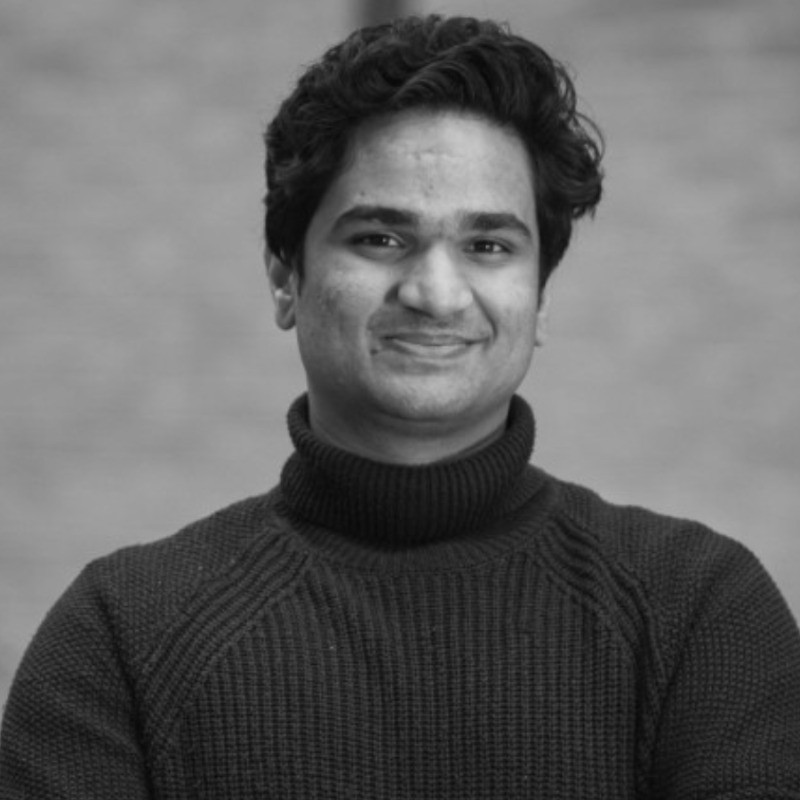
\includegraphics[width=2.0cm]{photo.jpg}
\end{minipage}
\vspace{-2pt}

% ================= SUMMARY =================
\section{Summary}
DevOps and Automation Engineer with 3+ years of experience engineering automated deployment pipelines, infrastructure automation, and resilient software delivery systems across European teams. At FlowSpace, orchestrated the zero-downtime platform and infrastructure migration off a legacy architecture onto a modern containerized Next.js, Laravel, and PostgreSQL stack, scaling from 2,000 to 4,500+ users. Proficient in designing automated CI/CD pipelines (Jenkins workflows, GitHub Actions), Infrastructure as Code with Terraform, configuration management with Ansible, Docker containerization, and advanced scripting in Python, Bash, and TypeScript.

% ================= SKILLS =================
\section{Skills}
\begin{itemize}
 \item \textbf{CI/CD \& Release Automation:} Jenkins pipelines, GitHub Actions workflows, automated build and deployment stages, branching strategies, PR management, artifact versioning, automated rollback, and blue-green/canary release concepts
 \item \textbf{Infrastructure as Code \& Cloud:} Terraform (IaC provisioning and state management), Cloud platforms (AWS, Azure, Supabase), Linux system administration, Docker containerization, cloud networking fundamentals, infrastructure security best practices
 \item \textbf{Configuration Management \& Scripting:} Ansible playbooks, server provisioning, environment configuration, Python scripting, Bash/Shell, TypeScript, Node.js, REST APIs, webhook automation, automated error recovery
 \item \textbf{Testing, Reliability \& Collaboration:} Automated end-to-end and integration testing (Playwright, Postman), unit testing, logging and observability, Git/GitHub, Jira, agile delivery in distributed multidisciplinary engineering teams
\end{itemize}

% ================= EXPERIENCE =================
\section{Experience}

\role{\href{https://flowspace.co}{FlowSpace.co}}{Mar 2024 - Aug 2026}{Lead DevOps \& Full-Stack Engineer (Full-time, Freelance)}{London, UK (remote)}
\begin{itemize}
 \item Led the core infrastructure and platform migration off a legacy stack onto containerized Next.js and Laravel (PostgreSQL) services, executing entity-level cutover scripts with zero downtime while scaling to 4,500+ users.
 \item Designed and maintained automated CI/CD pipelines and deployment workflows, automating testing, linting, and build steps to ensure reliable, repeatable releases across staging and production environments.
 \item Engineered custom Python and TypeScript automation scripts and webhook listeners to integrate external enterprise APIs (OfficeRnD, Nexudus), implementing automated retry logic, error handling, and transactional consistency.
 \item Architected an automated document ingestion pipeline (TypeScript, Python, n8n, Claude API) processing 900+ entities with schema-enforced validation, error logging, and human-in-the-loop review controls.
 \item Built automated end-to-end regression test suites with Playwright, embedding automated smoke tests into deployment pipelines to safeguard system stability.
\end{itemize}

\role{\href{https://get2germany.com}{Get2Germany.com}}{Jan 2024 - May 2024}{Developer \& Automation Specialist (Part-time)}{Berlin, Germany}
Developed automated data workflows in n8n, integrated Google Cloud APIs, and automated database maintenance and query optimization routines.\\[1pt]

\role{\href{https://clubee.com}{Clubee.com}}{Sep 2023 - Aug 2024}{Developer \& QA Automation (Full-time, Freelance)}{Foetz, Luxembourg}
Integrated enterprise REST APIs across the platform, maintained automated QA test suites, and developed administrative federation dashboard tools.\\[1pt]

\role{\href{https://tractionboard.co}{Tractionboard.co}}{Aug 2023 - Oct 2023}{Developer (Internship)}{Utrecht, Netherlands}
Integrated OpenAI and SendGrid APIs for automated data handling, resolved production bugs, and implemented responsive frontend interfaces.

% ================= SELECTED PROJECTS =================
\section{Selected Projects}
\begin{itemize}
 \item \textbf{\href{https://smarturlink.com/}{Urlink}} (2025), DevOps \& Full-Stack Engineer. Provisioned PostgreSQL schemas on Supabase, designed platform business logic, and automated continuous deployment workflows via Netlify CI/CD.
 \item \textbf{\href{https://ultrastrategy.com}{UltraStrategy}} (2024 - 2025), Automation Developer. Built an automated document-processing ETL pipeline using n8n and Eden AI for multi-source data extraction into structured candidate profiles.
 \item \textbf{\href{https://github.com/prab-gupta/llm-doc-parser}{LLM Document Parser}} (Open Source), Creator. Engineered a public pipeline parsing semi-structured documents into strictly validated JSON schemas with automated test coverage.
\end{itemize}

% ================= CERTIFICATIONS =================
\section{Certifications}
Microsoft Power Automate (Certified) \textbullet\ Microsoft Copilot Studio Agent Academy \textbullet\ Microsoft: Introduction to building AI agents \textbullet\ Tray.AI Build Practitioner (Sep 2024)

% ================= EDUCATION =================
\section{Education}
\textbf{Ca' Foscari University of Venice} \hfill Oct 2020 - Jun 2024\\
BA Philosophy, International Studies \& Economics (Minor: Entrepreneurship)

% ================= AUTH =================
\vspace{2pt}
{\small \textbf{Work authorization:} European Long Term Residence Permit (Italy); full authorization to work across Sweden and the EU without visa sponsorship; available immediately. \quad \textbf{Languages:} English (fluent / C2), Hindi (native), Italian (conversational).}

\end{document}
